\documentclass[]{elsarticle} %review=doublespace preprint=single 5p=2 column
%%% Begin My package additions %%%%%%%%%%%%%%%%%%%
\usepackage[hyphens]{url}



\usepackage{lineno} % add
\providecommand{\tightlist}{%
  \setlength{\itemsep}{0pt}\setlength{\parskip}{0pt}}

\usepackage{graphicx}
\usepackage{booktabs} % book-quality tables
%%%%%%%%%%%%%%%% end my additions to header

\usepackage[T1]{fontenc}
\usepackage{lmodern}
\usepackage{amssymb,amsmath}
\usepackage{ifxetex,ifluatex}
\usepackage{fixltx2e} % provides \textsubscript
% use upquote if available, for straight quotes in verbatim environments
\IfFileExists{upquote.sty}{\usepackage{upquote}}{}
\ifnum 0\ifxetex 1\fi\ifluatex 1\fi=0 % if pdftex
  \usepackage[utf8]{inputenc}
\else % if luatex or xelatex
  \usepackage{fontspec}
  \ifxetex
    \usepackage{xltxtra,xunicode}
  \fi
  \defaultfontfeatures{Mapping=tex-text,Scale=MatchLowercase}
  \newcommand{\euro}{€}
\fi
% use microtype if available
\IfFileExists{microtype.sty}{\usepackage{microtype}}{}
\bibliographystyle{elsarticle-harv}
\usepackage{longtable}
\ifxetex
  \usepackage[setpagesize=false, % page size defined by xetex
              unicode=false, % unicode breaks when used with xetex
              xetex]{hyperref}
\else
  \usepackage[unicode=true]{hyperref}
\fi
\hypersetup{breaklinks=true,
            bookmarks=true,
            pdfauthor={},
            pdftitle={Pervasive duplication of tumor suppressor genes preceded parallel evolution of large bodied Atlantogenatans},
            colorlinks=false,
            urlcolor=blue,
            linkcolor=magenta,
            pdfborder={0 0 0}}
\urlstyle{same}  % don't use monospace font for urls

\setcounter{secnumdepth}{0}
% Pandoc toggle for numbering sections (defaults to be off)
\setcounter{secnumdepth}{0}


% Pandoc header
\usepackage{longtable}
\usepackage{booktabs}
\usepackage{geometry}
\usepackage{pdflscape}



\begin{document}
\begin{frontmatter}

  \title{Pervasive duplication of tumor suppressor genes preceded parallel
evolution of large bodied Atlantogenatans}
    \author[University of Chicago]{Juan Manuel Vazquez}
  
    \author[SUNY Buffalo]{Vincent J Lynch}
  
      \address[University of Chicago]{Department of Human Genetics, 920 East 58th St, Chicago, IL, 60637}
    \address[SUNY Buffalo]{Department of Biological Sciences, 551 Cooke Hall, Buffalo NY, 14260}
    
  \begin{abstract}
  Cancer is an intrinsic disease of multicellular organisms. Within a
  species, the size of an animal, - correlated with the individual's
  number of cells - and its lifespan - correlated with increasing cellular
  damage over time - positively correlate with the risk any individual has
  to form tumors. Between species, however, we do not observe any
  correlation between size, lifespan, and cancer, a phenomenon that
  referred to as \emph{Peto's Paradox}. Elephants are a particularly
  interesting member of this class of paradoxical animals, since they are
  a set of large species deeply nested in a clade of smaller species,
  indicating a recent gain of size. Recent work has identified several
  individual cases of gene duplicates contributing to the increased cancer
  resistance of elephants, which suggests that duplication of tumor
  suppressor genes may play a more general role in mediating Peto's
  Paradox by increasing cancer resistance in large, long-lived species. By
  using a Reciprocal Best-Hit BLAT search approach, we investigated copy
  numbers of all protein-coding genes in \emph{Atlantogenatan} genomes to
  see if there is any correlation between the copy number of duplicates
  and changes body size along the phylogenetic tree. From an initial set
  of 18,011 protein-coding genes in hg38, we identified a median of 13,880
  genes in \emph{Atlantogenatan} genomes, of which a median of 940 genes
  are duplicated. We find that, just as body size fluctuates throughout
  \emph{Atlantogenata}, genes involved in tumor suppressor pathways are
  also duplicated throughout the phylogenetic tree. Extant species of
  elephants, however, show active transcription of both canonical and
  duplicated copies of tummor suppressors that duplicated prior to and
  during their sudden increase in body size, suggesting that the
  duplication of tumor suppressor genes facilitates the evolution of
  increased body size by compensating for the increased cancer risk.
  \end{abstract}
  
 \end{frontmatter}

)

\hypertarget{introduction}{%
\section{Introduction}\label{introduction}}

One of the major constraints on the evolution of large body sizes in
animals is an increased risk of developing cancer. If all cells in all
organisms have a similar risk of malignant transformation and equivalent
cancer suppression mechanisms, organism with many cells should have a
higher prevalence of cancer than organisms with fewer cells. Consistent
with this expectation there is a strong positive correlation between
body size and cancer incidence within species, for example, human cancer
incidence increases with increasing adult height {[}1,2{]} and cancer
incidence is positively correlated with body size in dogs {[}3,4{]}.
There is no correlation, however, between body size and cancer risk
between species. This lack of correlation is often referred to as
`Peto's Paradox' {[}5--7{]}. While it is clear that a resolution to
Peto's Paradox must involve the evolution of enhanced cancer protection
alongside increases in body size and lifespan, the specific genetic,
molecular, and cellular mechanisms that underlie this resistance have
proven elusive. {[}8--12{]}.

Among the challenges for discovering how animals evolved enhanced cancer
protection mechanisms is identifying lineages in which large bodied
species are nested within species with small body sizes. Afrotherian
mammals are generally small-bodied, similarly to the prediced common
ancestor of Eutherian mammals. For example, maximum adult weights are
\textasciitilde{}70g in golden moles, \textasciitilde{}120g in tenrecs,
\textasciitilde{}170g in elephant shrews, \textasciitilde{}3kg in
hyraxes, and 60kg in aardvarks {[}13{]}. However, while these extant
species are relatively small, the fossil evidence demonstrates that
their ancestral lineages reached enormous sizes. For example, while
extant hyraxes are relatively small, the extinct Titanohyrax is
estimated to have weighted up to \textasciitilde{}1300kg {[}14{]}. The
largest members of Afrotheria, too, are dwarfed by the size of their
recent ancestors: extant cows manatees are large bodied
(\textasciitilde{}322-480kg) but are relatively small compared to the
extinct Stellar's sea cow which is estimated to have weight 8000-10000kg
{[}15{]}. Similarly African (4,800kg) and Asian elephants (3,200kg) are
the largest living elephant species, but are dwarfed by the truly
gigantic extinct Proboscideans such as Deinotherium
(\textasciitilde{}132,000kg), Mammut borsoni (110,000kg), and the Asian
straight-tusked elephant (\textasciitilde{}220,000kg), the largest known
land mammal {[}16{]}. These large-bodied Afrotherian lineages are nested
within small bodied species (Fig. 1) {[}17--20{]}, indicating that
gigantism independently evolved in hyraxes, sea cows, and elephants
(Paenungulates). Thus, Paenungulates are an excellent model system in
which to explore the mechanisms that underlie the evolution of large
body sizes and augmented cancer resistance.

Although many mechanisms can potentially resolve Peto's paradox, among
the most parsimonious routes to enhanced cancer resistance is through an
increased copy number of tumor suppressors. Such an example has been
seen in the case of candidate genes such as \emph{TP53} and \emph{LIF}
{[}12,21,22{]} as well as in studies involving a limited set of
candidate genes {[}23,24{]}. As these studies focus on \emph{a priori}
gene sets, however, it remains unknown whether this is a general,
genome-wide trend in Afrotherian genomes; and whether such a general
trend is associated with the recent increases in body size -- and
therefore expected cancer risk -- in these species.

Here, we trace the evolution of body mass and gene copy number variation
in Afrotherians in order to investigate whether gene duplications are
enriched in large, long-lived species for genes involved in known tumor
suppression pathways. Our estimates of the evolution of body mass,
similarly to previous studies {[}17--20{]}, show that large body masses
evolved in a step-wise manner, with major increases in body mass in the
Pseudoungulata (17kg), Paenungulata (25kg), Tethytheria (296kg), and
Proboscidea (4,100kg) stem-lineages. Furthermore, we see that the
ancestral body size increases in Hydracoidia and Sirenia were
independent events. To study the evolution of gene copy number, we used
a genome-wide Reciprocal Best BLAT Hit (RBBH) method to identify gene
duplications in Afrotherian genomes, and used maximum likelihood
(treating copy number as a discrete trait) to infer the lineages in
which those duplications occurred. We found gene duplications in
lineages with increased body mass were enriched in functions related to
tumor suppression, including regulation of the cell cycle, DNA damage
repair, and regulation of apoptosis. These data suggest that duplication
of tumor suppressors played a role in the evolution of large, long-lived
in Afrotherians.

\hypertarget{methods}{%
\section{Methods}\label{methods}}

\hypertarget{ancestral-body-size-reconstruction}{%
\subsection{Ancestral Body Size
Reconstruction}\label{ancestral-body-size-reconstruction}}

We built a time-calibrated supertree of Eutherian mammals by combining
the time-calibrated molecular phylogeny of Bininda-Emonds \emph{et al.}
{[}25{]} with the time-calibrated total evidence Afrotherian phylogeny
from Puttick and Thomas {[}20{]}. While the Bininda-Emonds \emph{et al.}
{[}25{]} phylogeny includes 1,679 species, only 34 are Afrotherian, and
no fossil data are included. The inclusion of fossil data from extinct
species is essential to ensure that ancestral state reconstructions of
body mass are not biased by only including extant species. This can lead
to inaccurate reconstructions, for example, if lineages convergently
evolved large body masses from a small bodied ancestor. In contrast, the
total evidence Afrotherian phylogeny of Puttick and Thomas {[}20{]}
includes 77 extant species and fossil data from 39 extinct species.
Therefore we replaced the Afrotherian clade in the Bininda-Emonds
\emph{et al.} {[}25{]} phylogeny with the Afrotherian phylogeny of
Puttick and Thomas {[}20{]} using Mesquite. Next, we jointly estimated
rates of body mass evolution and reconstructed ancestral states using a
generalization of the Brownian motion model that relaxes assumptions of
neutrality and gradualism by considering increments to evolving
characters to be drawn from a heavy-tailed stable distribution (the
``Stable Model'') {[}26{]}. The stable model allows for occasional large
jumps in traits and has previously been shown to out-perform other
models of body mass evolution, including standard Brownian motion
models, Ornstein--Uhlenbeck models, early burst maximum likelihood
models, and heterogeneous multi-rate models {[}26{]}.

\hypertarget{identification-of-duplicate-genes}{%
\subsection{Identification of Duplicate
Genes}\label{identification-of-duplicate-genes}}

\textbf{Reciprocal Best-Hit BLAT:} We developed a reciprocal best hit
BLAT (RBHB) pipeline to identify putative homologs and estimate gene
copy numbers across species (\textbf{Figure 1A}). The Reciprocal Best
Hit (RBH) search strategy is conceptually straightforward: 1) Given a
gene of interest \(G_A\) in a query genome \(A\), one searches a target
genome \(B\) for all possible matches to \(G_A\); 2) For each of these
hits, one then performs the reciprocal search in the original query
genome to identify the highest-scoring hit; 3) A hit in genome \(B\) is
defined as a homolog of gene \(G_A\) if and only if the original gene
\(G_A\) is the top reciprocal search hit in genome \(A\). We selected
BLAT {[}27{]} as our algorithm of choice, as this algorithm is sensitive
to highly simliar (\textgreater{}90\% identity) sequences, thus
identifying the highest-confidence homologs while minimizing many-to-one
mapping problems when searching for multiple genes. RBH performs similar
to other more complex methods of orthology prediction, and is
particularly good at identifying incomplete genes that may be fragmented
in low quality/poor assembled regions of the genome {[}28,29{]}.

\textbf{Effective Copy Number By Coverage:} In lower-quality genomes,
many genes are fragmented across multiple scaffolds, which results in
BLAT calling multiple hits when in reality there is only one gene. To
compensate for this, we came up with a novel statistic, Estimated Copy
Number by Coverage (ECNC), which averages the number of times we see
each nucleotides of a query sequence in a target genome over the total
number of nucleotides of the query sequence found overall in each target
genome (Supplementary Figure 1). This allows us to correct for genes
that have been fragmented across incomplete genomes, while also taking
into account missing sequences from the human query in the target
genome. Mathematically, this can be written as:\\
\[ ECNC = \frac{\sum_{n=1}^{l} C_n}{\sum_{n=1}^{l} bool(C_n)}\] where
\(n\) is a given nucleotide in the query, \(l\) is the total length of
the query, \(C_n\) is the number of instances that \(n\) is present
within a reciprocal best hit, and \(bool(C_n)\) is 1 if \(C_n > 0\) or 0
if \(C_n = 0\).

\textbf{RecSearch Pipeline:} We created a custom Python pipeline for
automating RBHB searches between a single reference genome and multiple
target genomes using a list of query sequences from the reference
genome. For the query sequences in our search, we used the hg38 Proteome
provided by UniProt {[}30{]}, which is a comprehensive set of protein
sequences curated from a combination of predicted and validated protein
sequences generated by the UniProt Consortium. In order to refine our
search, we omitted protein sequences originating from long, noncoding
RNA loci (e.g.~LINC genes); poorly-studied genes from predicted open
reading frames (C-ORFs); and sequences with highly repetitive sequences
such as zinc fingers, protocadherins, and transposon-containing genes,
as these were prone to high levels of false positive hits.

After filtering out problematic protein queries (see ``Query gene
inclusion criteria''), we then used our pipeline (Figure 1A) to search
for all copies of our 18011 query genes in publicly available
Afrotherian genomes, including African savannah elephant
(\emph{Loxodonta africana}: loxAfr3, loxAfr4, loxAfrC), African forest
elephant (\emph{Loxodonta cyclotis}: loxCycF), Asian Elephant
(\emph{Elephas maximus}: eleMaxD), Woolly Mammoth (\emph{Mammuthus
primigenius}: mamPriV), Colombian mammoth (\emph{Mammuthus columbi}:
mamColU), American mastodon (\emph{Mammut americanum}: mamAmeI), Rock
Hyrax (\emph{Procavia capensis}: proCap1, proCap2, proCap2\_HiC), West
Indian Manatee (\emph{Trichechus manatus latirostris}: triManLat1,
triManLat1\_HiC), Aardvark (\emph{Orycteropus afer}: oryAfe1,
oryAfe1\_HiC), Lesser Hedgehog Tenrec (\emph{Echinops telfairi}:
echTel2), Nine-banded armadillo (\emph{Dasypus novemcinctus}: dasNov3),
Hoffman's two-toed sloth (\emph{Choloepus hoffmannii}: choHof1, choHof2,
choHof2\_HiC), Cape golden mole (\emph{Chrysochloris asiatica}:
chrAsi1), and Cape elephant shrew (\emph{Elephantulus edwardii}:
eleEdw1). For many of these species, we covered multiple assemblies in
order to test the effects of assembly size and quality on our hits.

\textbf{Query gene inclusion criteria:} To assemble our query list, we
first removed all unnamed genes from UP000005640. Next, we excluded
genes from downstream analyses for which assignment of homology was
uncertain, including uncharacterized ORFs (991), LOC (63), HLA genes
(402), replication dependent histones (72), odorant receptors (499),
ribosomal proteins (410), zinc finger transcription factors (1983),
viral and repetitive-element-associated proteins (82) and any protein
described as either ``Uncharacterized,'' ``Putative,'' or ``Fragment''
by UniProt in UP000005640 (30724), leaving us with a final set of 37582
query protein sequences, corresponding to 18011 genes.

\textbf{Duplication gene inclusion criteria:} In order to condense
transcript-level hits into single gene loci, and to resolve many-to-one
genome mappings, we removed exons where transcripts from different genes
overlapped, and merged overlapping transcripts of the same gene into a
single gene locus call. The resulting gene-level copy number table was
then combined with the maximum ECNC values observed for each gene in
order to call gene duplications. We called a gene duplicated if its copy
number was two or more, and if the maximum ECNC value of all the gene
transcripts searched was 1.5 or greater; previous studies have shown
that incomplete duplications can encode functional genes {[}12,22{]},
therefore partial gene duplications were included provided they passed
additional inclusion criteria. The ECNC cut off of 1.5 was selected
empirically, as this value minimized the number of false positives seen
in a test set of genes and genomes. The results of our initial search
are summarized in Figure 1B. Overall, we identified 13880 genes across
all species, or 77.1\% of our starting query genes.

\textbf{Genome Quality Assessment using CEGMA:} In order to determine
the effect of genome quality on our results, we used the gVolante
webserver and CEGMA to assess the quality and completeness of the genome
{[}31,32{]}. CEGMA was run using the default settings for mammals
(``Cut-off length for sequence statistics and composition'' = 1;``CEGMA
max intron length'' = 100000; ``CEGMA gene flanks'' = 10000, ``Selected
reference gene set'' = CVG). For each genome, we generated a correlation
matrix using the aforementioned genome quality scores, and either the
mean Copy Number or mean ECNC for all hits in the genome.

\hypertarget{evidence-for-functionality-of-identified-genes}{%
\subsection{Evidence for Functionality of Identified
Genes}\label{evidence-for-functionality-of-identified-genes}}

To validate and filter out duplicate gene calls, we intersected our
results with either gene prediction or transcriptomic evidence as a
proxy for functionality.

\textbf{Transcriptome Assembly:} For the African Savana Elephant, Asian
Elephant, West Indian Manatee, and Nine-Banded Armadillo, we generated
\emph{de novo} transcriptomes using publically-available RNA-sequencing
data from NCBI SRA (Supplementary Table 1). We mapped reads to all
genomes available for each species, and assembled transcripts using
HISAT2 and StringTie, respectively {[}33--35{]}. RNA-sequencing data was
not available for Cape Golden Mole, Cape Elephant Shrew, Rock Hyrax,
Aardvark, or the Lesser Hedgehog Tenrec.

\textbf{Gene Prediction:} We obtained tracks for genes predicted using
GenScan for all the genomes available via UCSC Genome Browser: African
savannah elephant (loxAfr3), Rock Hyrax (proCap1), West Indian Manatee
(triManLat1), Aardvark (oryAfe1), Lesser Hedgehog Tenrec (echTel2),
Nine-banded armadillo (dasNov3), Hoffman's Two-Toed Sloth (choHof1),
Cape golden mole (chrAsi1), and Cape Elephant Shrew (eleEdw1); gene
prediction tracks for higher-quality assemblies were not available.

\textbf{Evidenced Duplicate Criteria:} We intersected our records of
duplicate hits identified in each genome with the gene prediction tracks
and/or transcriptome assemblies using \texttt{bedtools}. When multiple
lines of evidence for functionality were present for a genome, we used
the union of all intersections as the final output for evidenced
duplicates. When analyzing the highest-quality assemblies available for
each species, if a species had neither gene prediction tracks nor
RNA-seq data for the highest-quality genome available, we conservatively
included all hits for the genome in the final set of evidenced
duplicates.

\hypertarget{reconstruction-of-ancestral-copy-numbers}{%
\subsection{Reconstruction of Ancestral Copy
Numbers}\label{reconstruction-of-ancestral-copy-numbers}}

We implemented a maximum likelihood method for determining the ancestral
copy numbers of genes in \emph{Atlantogenata} using IQ-Tree. For this
analysis, we used an unrooted species tree including only the
aforementioned \emph{Atlantogenata} species. We generated PHYLIP files
containing the copy number of each gene in the highest quality genome
for each species, encoding genes on a scale from 1-31+ copies as 1-9,
A-V; and encoding a gene's copy number as uncetain (``?'') when we did
not identify it in the genome. We used the included tree-searching and
model-testing functionality in IQ-Tree to determine the most likely
topology for the species tree, and to obtain the most likely model for
copy number changes in the genome. The most likely model for the
evolution of copy number was inferred to be a Jukes-Cantor type model
for morphological data with equal state frequencies, allowing for a
proportion of invariable sites, and using a discrete Gamma model with 4
rate categories. (``MK+FQ+I+G4''). We defined the ancestral state of a
node if it had greater than an 80\% posterior probability.

\hypertarget{pathway-enrichment-analysis}{%
\subsection{Pathway Enrichment
Analysis}\label{pathway-enrichment-analysis}}

To determine which pathways were associated with duplicated genes in
each species and lineage, we used WEBGESTALT to perform
overrepresentation analysis (ORA) of the duplicated gene lists relative
to our initial query gene list {[}36{]}. For the database of pathways
used in the analysis, we used Reactome {[}37{]}, Wikipathways, {[}38{]},
and KEGG {[}39{]}. For the ORA, we used FDR for determining
significance, and ran the analysis at FDR=0.1, FDR=0.2, FDR=0.3, and
FDR=0.5.

\hypertarget{lifespan-phylogenetic-least-square-regression-and-calculating-estimated-cancer-risk-thoughout-atlantogenata}{%
\subsection{Lifespan Phylogenetic Least-Square Regression and
Calculating Estimated Cancer Risk Thoughout
Atlantogenata}\label{lifespan-phylogenetic-least-square-regression-and-calculating-estimated-cancer-risk-thoughout-atlantogenata}}

In order to determine the cancer risk \(K\) at each node, we first
needed to calcultate ancestral lifespans at each node. To do so, we used
a Phylogenetic Generalized Least-Square Regression (PGLS) {[}40,41{]} to
calculate estimated ancestral lifespans across \emph{Atlantogenata}
using our estimates for body size at each node.

Next, we used a simplified multistage cancer risk model for body size
\(D\) and lifespan \(t\): \(K \approx Dt^6\) {[}7,42--44{]}. To
determine the change in \(K\) between nodes, we obtained the ratio
between the cancer risk \(K_{1}\) at any given node, and the cancer risk
\(K_{2}\) at its ancestral node, using the equation
\(\frac{K_{2}}{K_{1}} \approx \frac{D_{1}t_{1}^6}{D_{2}t_{2}^6}\).
Finally, to simplify comparisons, we calculated the fold change cancer
risk between a node and its ancestor as
\(\log_{2}(\frac{K_{2}}{K_{1}})\).

\hypertarget{results}{%
\section{Results}\label{results}}

\hypertarget{body-size-frequently-and-independently-expands-and-contracts-throughout-atlantogenata}{%
\subsection{\texorpdfstring{Body size frequently and independently
expands and contracts throughout
\emph{Atlantogenata}}{Body size frequently and independently expands and contracts throughout Atlantogenata}}\label{body-size-frequently-and-independently-expands-and-contracts-throughout-atlantogenata}}

\begin{figure}

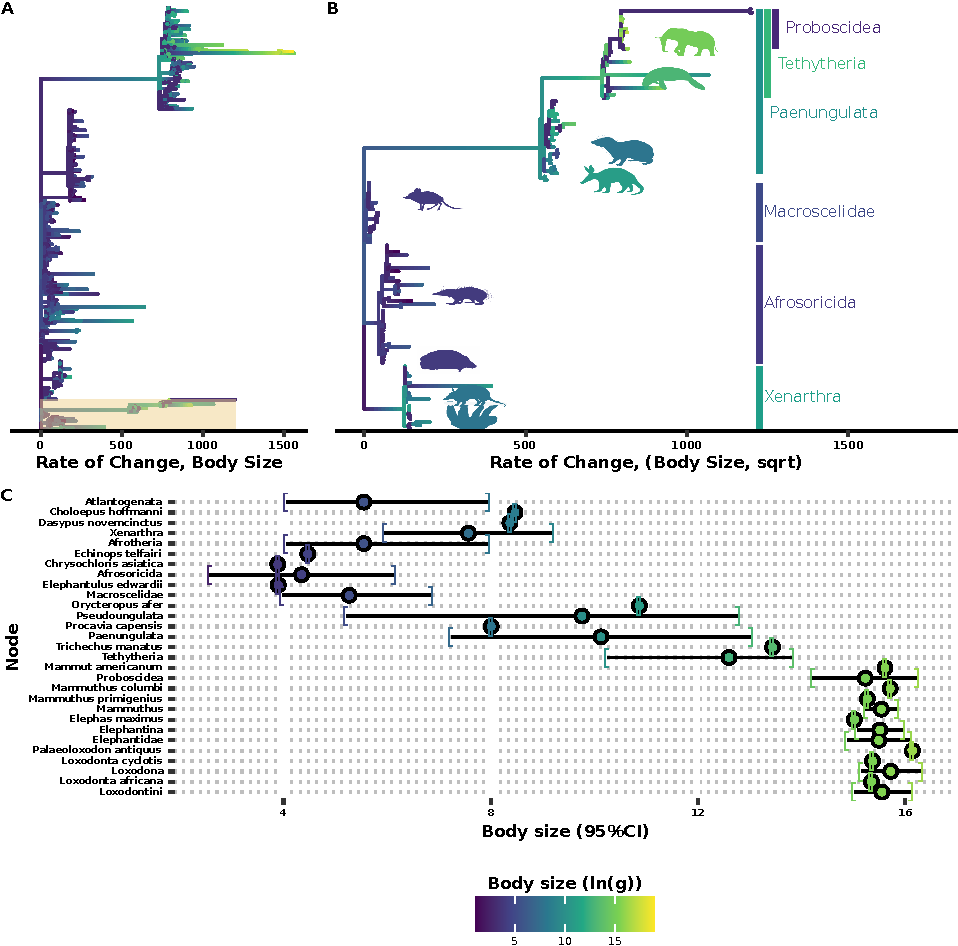
\includegraphics[width=6in]{paper_PLOS_draft_files/figure-latex/Figure1-1} \hfill{}

\caption{Body sizes rapidly and frequently expand in Eutherians, especially in Atlantogenata. **A)** Tree of Eutherian species, colored by ln(Body Size) and with branch lengths set to the rate of change in body sizes, normalized by the square root of the root branch. Atlantogenata is highlighted at the bottom. **B)** Zoom-in of (**A**) on Atlantogenata. Silhuetes for the African Elephant, West Indian Manatee, Cape Elephant Shrew, Lesser Hedgehog Tenrec, Cape Golden Mole, Nine-Banded Armadillo, and Hoffman's Two-Toed Sloth are colored by their extant body sizes, while clade labels are colored based on the common ancestor's estimated body size. **C)** Confidence interval plot for representative species and ancestral nodes.}\label{fig:Figure1}
\end{figure}

To trace the evolutionary history of body mass and lifespan in
Afrotherians, we built a time-calibrated supertree of Eutherian mammals
combining 1,679 species from Bininda-Emonds et al {[}25{]} with a total
evidence Afrotherian phylogeny including 77 extant and fossil data from
39 extinct species {[}20{]}. Fossil data from extinct species were
included to ensure that ancestral state reconstructions of body mass in
Afrotherians were not biased by only including extant species, which can
lead to inaccurate reconstructions, for example, if lineages multiple
lineages evolved large body masses from a small bodied ancestor. We
jointly estimated rates of body mass evolution and reconstructed
ancestral states using a generalization of a Brownian model of character
evolution, which allows for occasional large jumps in traits (stable
model) and out performs standard Brownian motion and Ornstein-Uhlenbeck
models of character evolution {[}26{]}.

Similar to previous studies of Afrotherian body size {[}20,26{]}, we
found that the body mass of the Afrotherian ancestor was inferred to be
small (0.26kg, 95\% CI: 0.31-3.01kg) and that substantial accelerations
in the rate of body mass evolution occurred coincident with a 67.36x
increase in body mass in the stem-lineage of \emph{Pseudoungulata}
(17.33kg), a 1.45x increase in body mass in the stem-lineage of
\emph{Paenungulata} (25.08kg), a 11.82x increase in body mass in the
stem-lineage of \emph{Tehthytheria} (296.56kg), and a 2.69x increase in
body mass in the stem-lineage of \emph{Proboscidea} (4114.39kg) (Figure
1B,C). The ancestral \emph{Hyracoidea} was inferred to be relatively
small 2.86kg-118.18kg, and rate accelerations were coincident with
independent body mass increases in large hyraxes such as
\emph{Titanohyrax andrewsi} 429.34kg; 67.36x increase. While the body
mass of the ancestral \emph{Sirenian} was inferred to be large
61.7kg-955.51kg, a rate acceleration occurred coincident with a 10.59x
increase in body mass in Stellar's sea cow. Rate accelerations also
occurred coincident with 36.6x decrease in body mass in the stem-lineage
of the dwarf elephants \emph{Elephas (Palaeoloxodon) antiquus falconeri}
and \emph{Elephas cypriotes}. These data suggest that gigantism in
\emph{Afrotherians} evolved step-wise, from small to medium bodies in
the \emph{Pseudoungulata} stem-lineage, medium to large bodies in the
\emph{Tehthytherian} stem-lineage and extinct hyraxes, and from large to
exceptionally large bodies independently in the \emph{Proboscidean}
stem-lineage and Stellar's sea cow (Figure 1).

\hypertarget{step-wise-reduction-of-intrinsic-cancer-risk-in-large-long-lived-afrotherians}{%
\subsection{Step-wise reduction of intrinsic cancer risk in large,
long-lived
Afrotherians}\label{step-wise-reduction-of-intrinsic-cancer-risk-in-large-long-lived-afrotherians}}

\begin{figure}

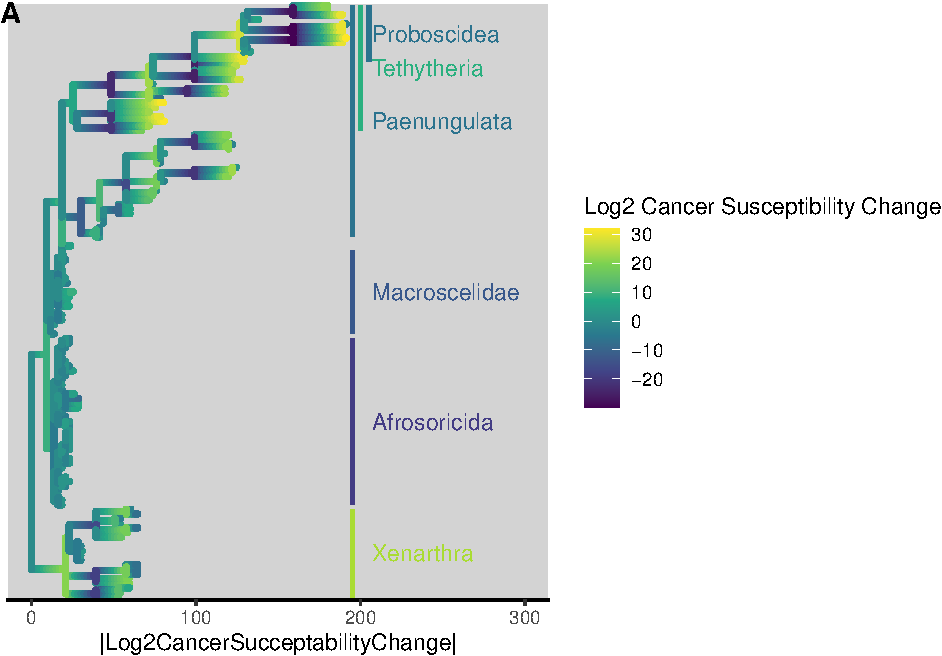
\includegraphics[width=6in]{paper_PLOS_draft_files/figure-latex/Figure2-1} \hfill{}

\caption{Cancer succecptibility across Atlantogenata}\label{fig:Figure2}
\end{figure}

\begin{longtable}[]{@{}lrlllr@{}}
\caption{Estimated Cancer Succeptibilty for nodes in
Atlantogenata}\tabularnewline
\toprule
Node & Est. Lifespan & K1 & K2 & Change in K & log2
Change\tabularnewline
\midrule
\endfirsthead
\toprule
Node & Est. Lifespan & K1 & K2 & Change in K & log2
Change\tabularnewline
\midrule
\endhead
Loxodontini & 34.38 & 1.47e+16 & 2.97e+15 & 4.94e+00 &
2.31\tabularnewline
Loxodonta africana & 65.00 & 2.47e+17 & 1.47e+16 & 1.68e+01 &
4.07\tabularnewline
Loxodona & 34.38 & 1.47e+16 & 1.47e+16 & 1.00e+00 & 0.00\tabularnewline
Loxodonta cyclotis & 31.12 & 2.97e+15 & 1.47e+16 & 2.02e-01 &
-2.31\tabularnewline
Palaeoloxodon antiquus & 34.38 & 1.47e+16 & 1.47e+16 & 1.00e+00 &
0.00\tabularnewline
Elephantidae & 31.12 & 2.97e+15 & 1.40e+07 & 2.13e+08 &
27.66\tabularnewline
Elephantina & 34.38 & 1.47e+16 & 2.97e+15 & 4.94e+00 &
2.31\tabularnewline
Elephas maximus & 65.50 & 2.58e+17 & 1.47e+16 & 1.76e+01 &
4.14\tabularnewline
Mammuthus & 34.38 & 1.47e+16 & 1.47e+16 & 1.00e+00 & 0.00\tabularnewline
Mammuthus primigenius & 31.12 & 2.97e+15 & 1.47e+16 & 2.02e-01 &
-2.31\tabularnewline
Mammuthus columbi & 34.38 & 1.47e+16 & 1.47e+16 & 1.00e+00 &
0.00\tabularnewline
Proboscidea & 9.41 & 1.40e+07 & 1.21e+14 & 1.15e-07 &
-23.05\tabularnewline
Mammut americanum & 34.38 & 1.47e+16 & 1.40e+07 & 1.05e+09 &
29.97\tabularnewline
Tethytheria & 25.49 & 1.21e+14 & 1.01e+12 & 1.21e+02 &
6.92\tabularnewline
Trichechus manatus & 69.00 & 4.77e+16 & 1.21e+14 & 3.93e+02 &
8.62\tabularnewline
Paenungulata & 18.91 & 1.01e+12 & 1.01e+12 & 1.00e+00 &
0.00\tabularnewline
Procavia capensis & 14.80 & 3.13e+10 & 1.01e+12 & 3.11e-02 &
-5.01\tabularnewline
Pseudoungulata & 18.91 & 1.01e+12 & 1.69e+09 & 5.97e+02 &
9.22\tabularnewline
Orycteropus afer & 29.80 & 4.19e+13 & 1.01e+12 & 4.17e+01 &
5.38\tabularnewline
Elephantulus edwardii & 10.40 & 6.90e+07 & 1.69e+09 & 4.09e-02 &
-4.61\tabularnewline
Afrosoricida & 10.40 & 6.90e+07 & 1.69e+09 & 4.09e-02 &
-4.61\tabularnewline
Chrysochloris asiatica & 10.40 & 6.90e+07 & 6.90e+07 & 1.00e+00 &
0.00\tabularnewline
Echinops telfairi & 19.00 & 2.57e+09 & 6.90e+07 & 3.72e+01 &
5.22\tabularnewline
Afrotheria & 12.69 & 1.69e+09 & 2.83e+06 & 5.97e+02 &
9.22\tabularnewline
Xenarthra & 20.89 & 4.97e+12 & 2.83e+06 & 1.76e+06 &
20.75\tabularnewline
Dasypus novemcinctus & 22.30 & 3.67e+11 & 4.97e+12 & 7.37e-02 &
-3.76\tabularnewline
Choloepus hoffmanni & 41.00 & 1.42e+13 & 4.97e+12 & 2.85e+00 &
1.51\tabularnewline
Atlantogenata & 8.52 & 2.83e+06 & 2.83e+06 & 1.00e+00 &
0.00\tabularnewline
Afroinsectivora & 12.69 & 1.69e+09 & 1.69e+09 & 1.00e+00 &
0.00\tabularnewline
\bottomrule
\end{longtable}

The dramatic increase in body mass and lifespan in some Afrotherian
lineages implies those lineages evolved reduced cancer risk. To infer
the magnitude of these reductions we estimated differences in cancer
risk between small bodied, short-lived species and large bodied,
long-lived species as well as for reconstructed ancestral Afrotherians.
Following {[}44{]} we estimate the intrinsic cancer risk as the product
of risk associated with body mass and lifespan. Differences in cancer
susceptibility \(K\) due to body mass differences between species can be
approximated simply as the fold difference in body mass (\(D\)) between
species {[}44{]}. The risk of developing cancer also increases in
proportion to the sixth power of age and is approximated by the formula
\(Ct^6\), in which the proportionality constant C that determines
susceptibility to cancer induction is multiplied by the sixth power of
the age in years, \(t\) {[}44--46{]}. Thus we can estimate the intrinsic
cancer risk for a species as \(K \approx Dt^6\).

In order to estimate the intrinsic cancer risk of a species, we first
obtained estimates for lifespans at ancestral nodes using PGLS and the
model
\(ln(lifespan) = \beta_{1}corBrownian +\beta_{2}ln(Size) + \epsilon\)
(Table 2). With this information in hand, we calculated \(K_{1}\) at all
nodes, and then estimated the fold change in cancer susceptibility
between an ancestral node and a given node as \(\frac{K_{2}}{K_{1}}\)
(\textbf{Table 4}). As body size and phylogeny are the strongest
predictors of lifespan, we find that this regression is sufficiently
robust without further metabolic or other covariates for our purposes
herein.

As shown in \textbf{Table 2}, cancer susceptibility skyrocketed at the
initial divergence of Atlantogenata, followed by a generally upwards
trend. At the common ancestor of Afrotheria there is an initial
9.22-fold increase in cancer risk. In parallel to Afrotheria, cancer
susceptibility increases 20.75-fold in Xenarthra. However, cancer risk
slowly deflates as size decreases as one moves along the tree towards
extant species, such as in Hoffman's Two Toed Sloth (1.51-fold change)
and in the Nine-banded Armadillo (-3.76-fold change).

Within Afrotheria, cancer susceptibility drops in Afrosoricida as
species shrink (-4.61-fold, then stagnates for the Cape Golden Mole) -
but then rises 5.22-fold towards the Lesser Hedgehog Tenrec. In
parallel, Afroinsectivora does not increase in cancer susceptibility,
and decreases once more at the Cape Elephant Shrew (-4.61-fold). The
emergence of Pseudoungulata sees the next big leap in cancer
susceptibility with a 9.22-fold increase. The Aardvark further increases
5.38-fold, while we don't observe an increase at the common ancestor of
Paenungulates. While the Rock Hyrax decreases in cancer susceptibility
as expected (-5.01-fold), Tethytheria sees a sharp increase in cancer
risk (6.92-fold). Within Tethytheria, the Manatee's cancer risk
increases once more 8.62-fold, while Proboscidea's cancer risk drops
precipitously along with its body size (-23.05-fold). Yet, within
Proboscidea we see the biggest increases: right off the bat, we see that
the cancer susceptibility of Elephantidae and the American Mastodon
skyrocket by 27.66-fold and 29.97-fold, respectively. Both Elephantina
and Loxodontini in Elephantidae have a 2.31-fold increase in cancer
susceptibility. Within Elephantina, cancer susceptibility stays stable
at Mammuthus and in the Colombian Mammoth, and slightly decreases in the
Wooly Mammoth (-2.31-fold). The three extant elephants - Asian Elephant
in Elephantina, the African Savana Elephant in Loxodontini, and the
African Forest Elephant in Loxodona, meanwhile, have parallel and
similar decreases in both size and cancer susceptibility (4.14-, 4.07-,
and -2.31-fold, respectively). Neither the common ancestor of Loxodonta,
nor the Straight-Tusked Mammoth see any further changes in cancer
susceptibility.

\hypertarget{identification-and-evolutionary-history-of-gene-duplications}{%
\subsection*{Identification and evolutionary history of gene
duplications}\label{identification-and-evolutionary-history-of-gene-duplications}}
\addcontentsline{toc}{subsection}{Identification and evolutionary
history of gene duplications}

\hypertarget{refs}{}
\leavevmode\hypertarget{ref-Green2011}{}%
1. Green J, Cairns BJ, Casabonne D, Wright FL, Reeves G, Beral V, et al.
Height and cancer incidence in the Million Women Study: prospective
cohort, and meta-analysis of prospective studies of height and total
cancer risk. The Lancet Oncology. 2011;12: 785--794.
doi:\href{https://doi.org/10.1016/s1470-2045(11)70154-1}{10.1016/s1470-2045(11)70154-1}

\leavevmode\hypertarget{ref-Nunney:20181c2}{}%
2. Nunney L. Size matters: height, cell number and a person's risk of
cancer. Proc R Soc B. 2018;285: 20181743.
doi:\href{https://doi.org/10.1098/rspb.2018.1743}{10.1098/rspb.2018.1743}

\leavevmode\hypertarget{ref-Dobson2013}{}%
3. Dobson JM. Breed-predispositions to cancer in pedigree dogs. ISRN
veterinary science. 2013;2013: 941275.
doi:\href{https://doi.org/10.1155/2013/941275}{10.1155/2013/941275}

\leavevmode\hypertarget{ref-Dorn1968}{}%
4. Dorn CR, Taylor DON, Schneider R, Hibbard HH, Klauber MR. Survey of
Animal Neoplasms in Alameda and Contra Costa Counties, California. II.
Cancer Morbidity in Dogs and Cats From Alameda County\textless{}xref
ref-type="fn" rid="FN2"\textgreater{}2\textless{}/xref\textgreater{}.
JNCI: Journal of the National Cancer Institute. 1968;40: 307--318.
doi:\href{https://doi.org/10.1093/jnci/40.2.307}{10.1093/jnci/40.2.307}

\leavevmode\hypertarget{ref-Caulin2011}{}%
5. Caulin AF, Maley CC. Peto's Paradox: evolution's prescription for
cancer prevention. Trends in ecology \& evolution. 2011;26: 175--82.
doi:\href{https://doi.org/10.1016/j.tree.2011.01.002}{10.1016/j.tree.2011.01.002}

\leavevmode\hypertarget{ref-Leroi2003}{}%
6. Leroi AM, Koufopanou V, Burt A. Cancer selection. Nature Reviews
Cancer. 2003;3: 226--231.
doi:\href{https://doi.org/10.1038/nrc1016}{10.1038/nrc1016}

\leavevmode\hypertarget{ref-Peto1975}{}%
7. Peto R, Roe F, Lee P, Levy L, Clack J. Cancer and ageing in mice and
men. British Journal of Cancer. 1975;32: 411--426.
doi:\href{https://doi.org/10.1038/bjc.1975.242}{10.1038/bjc.1975.242}

\leavevmode\hypertarget{ref-Ashur-Fabian2004}{}%
8. Ashur-Fabian O, Avivi A, Trakhtenbrot L, Adamsky K, Cohen M, Kajakaro
G, et al. Evolution of p53 in hypoxia-stressed Spalax mimics human tumor
mutation. Proceedings of the National Academy of Sciences. 2004;101:
12236--12241.
doi:\href{https://doi.org/10.1073/pnas.0404998101}{10.1073/pnas.0404998101}

\leavevmode\hypertarget{ref-Seluanov2008}{}%
9. Seluanov A, Hine C, Bozzella M, Hall A, Sasahara THC, Ribeiro AACM,
et al. Distinct tumor suppressor mechanisms evolve in rodent species
that differ in size and lifespan. Aging cell. 2008;7: 813--23.
doi:\href{https://doi.org/10.1111/j.1474-9726.2008.00431.x}{10.1111/j.1474-9726.2008.00431.x}

\leavevmode\hypertarget{ref-Gorbunova2012}{}%
10. Gorbunova V, Hine C, Tian X, Ablaeva J, Gudkov AV, Nevo E, et al.
Cancer resistance in the blind mole rat is mediated by concerted
necrotic cell death mechanism. Proceedings of the National Academy of
Sciences of the United States of America. 2012;109: 19392--6.
doi:\href{https://doi.org/10.1073/pnas.1217211109}{10.1073/pnas.1217211109}

\leavevmode\hypertarget{ref-Tian2013}{}%
11. Tian X, Azpurua J, Hine C, Vaidya A, Myakishev-Rempel M, Ablaeva J,
et al. High molecular weight hyaluronan mediates the cancer resistance
of the naked mole-rat. 2013;499.
doi:\href{https://doi.org/10.1038/nature12234}{10.1038/nature12234}

\leavevmode\hypertarget{ref-Sulak2015}{}%
12. Sulak M, Fong L, Mika K, Chigurupati S, Yon L, Mongan NP, et al.
TP53 copy number expansion is associated with the evolution of increased
body size and an enhanced DNA damage response in elephants. eLife.
2016;5: e11994.
doi:\href{https://doi.org/10.7554/elife.11994}{10.7554/elife.11994}

\leavevmode\hypertarget{ref-HAGR}{}%
13. Tacutu R, Craig T, Budovsky A, Wuttke D, Lehmann G, Taranukha D, et
al. Human Ageing Genomic Resources: Integrated databases and tools for
the biology and genetics of ageing. Nucleic Acids Research. 2013;41:
D1027--D1033.
doi:\href{https://doi.org/10.1093/nar/gks1155}{10.1093/nar/gks1155}

\leavevmode\hypertarget{ref-Schwartz1995}{}%
14. Schwartz GT, Rasmussen DT, Smith RJ. Body-Size Diversity and
Community Structure of Fossil Hyracoids. Journal of Mammalogy. 1995;76:
1088--1099. doi:\href{https://doi.org/10.2307/1382601}{10.2307/1382601}

\leavevmode\hypertarget{ref-Scheffer1972}{}%
15. Scheffer VB. The Weight of the Steller Sea Cow. Journal of
Mammalogy. 1972;53: 912--914.
doi:\href{https://doi.org/10.2307/1379236}{10.2307/1379236}

\leavevmode\hypertarget{ref-Larramendi:20151c2}{}%
16. Larramendi A. Shoulder Height, Body Mass, and Shape of
Proboscideans. Acta Palaeontologica Polonica. 2015;61.
doi:\href{https://doi.org/10.4202/app.00136.2014}{10.4202/app.00136.2014}

\leavevmode\hypertarget{ref-OLeary2013a}{}%
17. O'Leary MA, Bloch JI, Flynn JJ, Gaudin TJ, Giallombardo A, Giannini
NP, et al. The placental mammal ancestor and the post-K-Pg radiation of
placentals. Science (New York, NY). 2013;339: 662--7.
doi:\href{https://doi.org/10.1126/science.1229237}{10.1126/science.1229237}

\leavevmode\hypertarget{ref-Springer2013}{}%
18. Springer MS, Meredith RW, Teeling EC, Murphy WJ. Technical comment
on "The placental mammal ancestor and the post-K-Pg radiation of
placentals". Science (New York, NY). 2013;341: 613.
doi:\href{https://doi.org/10.1126/science.1238025}{10.1126/science.1238025}

\leavevmode\hypertarget{ref-OLeary2013b}{}%
19. O'Leary MA, Bloch JI, Flynn JJ, Gaudin TJ, Giallombardo A, Giannini
NP, et al. Response to comment on "The placental mammal ancestor and the
post-K-Pg radiation of placentals". Science (New York, NY). 2013;341:
613.
doi:\href{https://doi.org/10.1126/science.1238162}{10.1126/science.1238162}

\leavevmode\hypertarget{ref-PuttickAndThomas2015}{}%
20. Puttick MN, Thomas GH. Fossils and living taxa agree on patterns of
body mass evolution: a case study with Afrotheria. Proceedings
Biological sciences / The Royal Society. 2015;282: 20152023.
doi:\href{https://doi.org/10.1098/rspb.2015.2023}{10.1098/rspb.2015.2023}

\leavevmode\hypertarget{ref-Abegglen:JAMA2015}{}%
21. Abegglen LM, Caulin AF, Chan A, Lee K, Robinson R, Campbell MS, et
al. Potential Mechanisms for Cancer Resistance in Elephants and
Comparative Cellular Response to DNA Damage in Humans. JAMA. 2015;314:
1850--1860.
doi:\href{https://doi.org/10.1001/jama.2015.13134}{10.1001/jama.2015.13134}

\leavevmode\hypertarget{ref-Vazquez2018}{}%
22. Vazquez JM, Sulak M, Chigurupati S, Lynch VJ. A Zombie LIF Gene in
Elephants Is Upregulated by TP53 to Induce Apoptosis in Response to DNA
Damage. Cell Reports. 2018;24: 1765--1776.
doi:\href{https://doi.org/10.1016/j.celrep.2018.07.042}{10.1016/j.celrep.2018.07.042}

\leavevmode\hypertarget{ref-Caulin2015}{}%
23. Caulin AF, Graham TA, Wang L-S, Maley CC. Solutions to Peto's
paradox revealed by mathematical modelling and cross-species cancer gene
analysis. Philosophical transactions of the Royal Society of London
Series B, Biological sciences. 2015;370: 20140222.
doi:\href{https://doi.org/10.1098/rstb.2014.0222}{10.1098/rstb.2014.0222}

\leavevmode\hypertarget{ref-Doherty2016}{}%
24. Doherty A, Magalhães J de. Has gene duplication impacted the
evolution of Eutherian longevity? Aging Cell. 2016;15: 978--980.
doi:\href{https://doi.org/10.1111/acel.12503}{10.1111/acel.12503}

\leavevmode\hypertarget{ref-Bininda-Emonds2008}{}%
25. Bininda-Emonds ORP, Cardillo M, Jones KE, MacPhee RDE, Beck RMD,
Grenyer R, et al. Erratum: The delayed rise of present-day mammals.
Nature. 2008;456: 274--274.
doi:\href{https://doi.org/10.1038/nature07347}{10.1038/nature07347}

\leavevmode\hypertarget{ref-ElliotAndMooers2014}{}%
26. Elliot MG, Mooers AØ. Inferring ancestral states without assuming
neutrality or gradualism using a stable model of continuous character
evolution. BMC evolutionary biology. 2014;14: 226.
doi:\href{https://doi.org/10.1186/s12862-014-0226-8}{10.1186/s12862-014-0226-8}

\leavevmode\hypertarget{ref-blat}{}%
27. Kent JW. BLAT?The BLAST-Like Alignment Tool. Genome Research.
2002;12: 656--664.
doi:\href{https://doi.org/10.1101/gr.229202}{10.1101/gr.229202}

\leavevmode\hypertarget{ref-AltenhoffAndDessimoz2009}{}%
28. Altenhoff AM, Dessimoz C. Phylogenetic and functional assessment of
orthologs inference projects and methods. PLoS computational biology.
2009;5: e1000262.
doi:\href{https://doi.org/10.1371/journal.pcbi.1000262}{10.1371/journal.pcbi.1000262}

\leavevmode\hypertarget{ref-SalichosAndRokas2011}{}%
29. Salichos L, Rokas A. Evaluating ortholog prediction algorithms in a
yeast model clade. PloS one. 2011;6: e18755.
doi:\href{https://doi.org/10.1371/journal.pone.0018755}{10.1371/journal.pone.0018755}

\leavevmode\hypertarget{ref-uniprot}{}%
30. Consortium TU. UniProt: the universal protein knowledgebase. Nucleic
Acids Research. 2017;45: D158--D169.
doi:\href{https://doi.org/10.1093/nar/gkw1099}{10.1093/nar/gkw1099}

\leavevmode\hypertarget{ref-gVolante}{}%
31. Nishimura O, Hara Y, Kuraku S. gVolante for standardizing
completeness assessment of genome and transcriptome assemblies.
Bioinformatics. 2017;33: 3635--3637.
doi:\href{https://doi.org/10.1093/bioinformatics/btx445}{10.1093/bioinformatics/btx445}

\leavevmode\hypertarget{ref-CEGMA}{}%
32. Parra G, Bradnam K, Ning Z, Keane T, Korf I. Assessing the gene
space in draft genomes. Nucleic Acids Research. 2008;37: 289--297.
doi:\href{https://doi.org/10.1093/nar/gkn916}{10.1093/nar/gkn916}

\leavevmode\hypertarget{ref-HISAT}{}%
33. Kim D, Langmead B, Salzberg SL. HISAT: a fast spliced aligner with
low memory requirements. Nature Methods. 2015;12: 357--360.
doi:\href{https://doi.org/10.1038/nmeth.3317}{10.1038/nmeth.3317}

\leavevmode\hypertarget{ref-StringTie}{}%
34. Pertea M, Pertea GM, Antonescu CM, Chang T-C, Mendell JT, Salzberg
SL. StringTie enables improved reconstruction of a transcriptome from
RNA-seq reads. Nature Biotechnology. 2015;33: 290--295.
doi:\href{https://doi.org/10.1038/nbt.3122}{10.1038/nbt.3122}

\leavevmode\hypertarget{ref-Tuxedo}{}%
35. Pertea M, Kim D, Pertea GM, Leek JT, Salzberg SL. Transcript-level
expression analysis of RNA-seq experiments with HISAT, StringTie and
Ballgown. Nature Protocols. 2016;11: 1650--1667.
doi:\href{https://doi.org/10.1038/nprot.2016.095}{10.1038/nprot.2016.095}

\leavevmode\hypertarget{ref-WebGestalt2019}{}%
36. Liao Y, Wang J, Jaehnig EJ, Shi Z, Zhang B. WebGestalt 2019: gene
set analysis toolkit with revamped UIs and APIs. Nucleic Acids Research.
2019;47: W199--W205.
doi:\href{https://doi.org/10.1093/nar/gkz401}{10.1093/nar/gkz401}

\leavevmode\hypertarget{ref-Reactome}{}%
37. Jassal B, Matthews L, Viteri G, Gong C, Lorente P, Fabregat A, et
al. The reactome pathway knowledgebase. Nucleic acids research. 2020;48:
D498--D503.
doi:\href{https://doi.org/10.1093/nar/gkz1031}{10.1093/nar/gkz1031}

\leavevmode\hypertarget{ref-Wikipathways}{}%
38. Slenter DN, Kutmon M, Hanspers K, Riutta A, Windsor J, Nunes N, et
al. WikiPathways: a multifaceted pathway database bridging metabolomics
to other omics research. Nucleic Acids Research. 2017;46: D661--D667.
doi:\href{https://doi.org/10.1093/nar/gkx1064}{10.1093/nar/gkx1064}

\leavevmode\hypertarget{ref-KEGG}{}%
39. Kanehisa M, Goto S. KEGG: Kyoto Encyclopedia of Genes and Genomes.
Nucleic Acids Research. 2000;28: 27--30.
doi:\href{https://doi.org/10.1093/nar/28.1.27}{10.1093/nar/28.1.27}

\leavevmode\hypertarget{ref-Felsenstein1985}{}%
40. Felsenstein J. Phylogenies and the Comparative Method. The American
Naturalist. 1985;125: 1--15.
doi:\href{https://doi.org/10.1086/284325}{10.1086/284325}

\leavevmode\hypertarget{ref-MartinsAndHansen1997}{}%
41. Martins EP, Hansen TF. Phylogenies and the Comparative Method: A
General Approach to Incorporating Phylogenetic Information into the
Analysis of Interspecific Data. The American Naturalist. 1997;149:
646--667. doi:\href{https://doi.org/10.1086/286013}{10.1086/286013}

\leavevmode\hypertarget{ref-Armitage:19851c2}{}%
42. Armitage P. Multistage models of carcinogenesis. Environmental
health perspectives. 1985;63: 195--201.
doi:\href{https://doi.org/10.1289/ehp.8563195}{10.1289/ehp.8563195}

\leavevmode\hypertarget{ref-Armitage:20041c2}{}%
43. Armitage P, Doll R. The age distribution of cancer and a multi-stage
theory of carcinogenesis. British Journal of Cancer. 2004;91: 6602297.
doi:\href{https://doi.org/10.1038/sj.bjc.6602297}{10.1038/sj.bjc.6602297}

\leavevmode\hypertarget{ref-Peto:20151c2}{}%
44. Peto R. Quantitative implications of the approximate irrelevance of
mammalian body size and lifespan to lifelong cancer risk. Phil Trans R
Soc B. 2015;370: 20150198.
doi:\href{https://doi.org/10.1098/rstb.2015.0198}{10.1098/rstb.2015.0198}

\leavevmode\hypertarget{ref-ArmitageAndDoll1954}{}%
45. Armitage P, Doll R. The Age Distribution of Cancer and a Multi-stage
Theory of Carcinogenesis. British Journal of Cancer. 1954;8: 1--12.
doi:\href{https://doi.org/10.1038/bjc.1954.1}{10.1038/bjc.1954.1}

\leavevmode\hypertarget{ref-Nordling1953}{}%
46. Nordling CO. A New Theory on the Cancer-inducing Mechanism. British
Journal of Cancer. 1953;7: 68--72.
doi:\href{https://doi.org/10.1038/bjc.1953.8}{10.1038/bjc.1953.8}


\end{document}


